%-----------------------------------------------------------------------
% Cabecera del documento. Aqui se incluyen los paquetes y las
% definiciones que se utilizen despues en el documento.

\documentclass[a4paper,11pt]{article} % Tipo del documento. Puede ser
% book, article, report, y
% muchos mas

\usepackage{./estilos/estiloBase} % Basicamente son todas las
% librerias usadas. En caso de que
% falten librerias se van añadiendo
% al fichero.
\usepackage{./estilos/colores} % Algunos colores ya generados, para
% los algunos estilos más avanzados.
\usepackage{./estilos/comandos} % Algunos comandos personalizados

%\usepackage{./estilos/pygments}

\graphicspath{{./imagenes/}}

\title{Aplicación web para la gestión de la planificación docente de los grados} % Título del documento
\author{Alumno: Daniel Ignacio Salazar Recio\\Director: Juan José Domínguez Jiménez} % Autor (o
% autores)
\date{\today} % Fecha. La orden \today indica el dia de hoy con dia
% mes y año.

%----------------------------------------------------------------------

\begin{document} % Lo que este en el entorno document es lo que se va
% a mostrar finalmente.
%\sinmargen
\maketitle % Generacion automatica del titulo o la portada si es un book.

\abstract{\noindent El siguiente documento se presenta a modo de resumen que
complementa la Memoria del mismo Proyecto Fin de Carrera, entregada de forma
simultánea a este resumen. El proyecto consiste en una aplicación que permite configurar la carga global de las titulaciones de grado de la ESI, el calendario y los horarios, además de permitir la generación de informes.}

\tableofcontents % Genera automaticamente el indice. Es necesario
% compilar dos veces para que este salga.

\section{Introducción y motivaciones}
Con este Proyecto de Fin de Carrera se pretende la consecución de dos objetivos fundamentales: poner en práctica los conocimientos adquiridos en la titulación de Ingeniería Técnica en Informática de Sistemas y buscar un incremento de los conocimientos en la rama del desarrollo web, al no haber estudiado nada de este tema durante la carrera.
%%%%%%%%%%%%%%%%%%%%%%%%%%%%%%%%%%%%%%%%%%%%%%%%%%%%%%%%%%%%%%%%%%%%%%%%%%%%%%%
%%%%%%%%%%%%%%%%%%%%%%%%%%%%%%%%OBJETIVOS%%%%%%%%%%%%%%%%%%%%%%%%%%%%%%%%%%%%
%%%%%%%%%%%%%%%%%%%%%%%%%%%%%%%%%%%%%%%%%%%%%%%%%%%%%%%%%%%%%%%%%%%%%%%%%%%%%%%
\section{Objetivos}

\paragraph{}
El proyecto consiste en la creación de un software que ayude a los coordinadores de las titulaciones de grado a programar la planificación docente.
\paragraph{}
En principio está pensado únicamente para el contexto de la Escuela Superior de Ingeniería, aunque debería ser fácilmente adaptable a otras facultades.
\paragraph{}
Actualmente para hacer esta planificación se utilizan hojas de cálculo de {\em Microsoft Excel} o {\em OpenOffice}, haciendo que el trabajo sea algo tedioso al tener que comprobar multitud de factores manualmente. La aplicación pretende facilitar esta labor, realizando esas comprobaciones automáticamente. 
\paragraph{}
La aplicación permite cosas como la tarea de realizar un horario y comprobar que un aula no esté ya ocupada por otra asignatura. Para ello el objetivo es crear una aplicación web de código abierto.
\paragraph{}
Otro objetivo que se pretende con este proyecto es hacerlo escalable, para que en un futuro se le puedan realizar las ampliaciones necesarias sin necesidad de cambiar demasiado lo que está ya hecho.

%%%%%%%%%%%%%%%%%%%%%%%%%%%%%%%%%%%%%%%%%%%%%%%%%%%%%%%%%%%%%%%%%%%%%%%%%%%%%%%
%%%%%%%%%%%%%%%%%%%%%%%%%%%%%%%PLANIFICACION%%%%%%%%%%%%%%%%%%%%%%%%%%%%%%%%%%%
%%%%%%%%%%%%%%%%%%%%%%%%%%%%%%%%%%%%%%%%%%%%%%%%%%%%%%%%%%%%%%%%%%%%%%%%%%%%%%%
La planificación se divide en varias fases, a continuación se explicará en detalle cada una de ellas.

\subsection{Fase inicial}

La primera fase consistió en el planteamiento de la idea del proyecto, que en principio era desarrollar una aplicación web. El tutor finalmente decide proponer este proyecto, dejando al alumno la libre elección de las tecnologías utilizadas para su desarrollo.

\subsection{Fase de análisis}

Se realizan diversas reuniones con el tutor para hacer el planteamiento y una especificación informal de los requisitos. Debido a la complejidad de la aplicación fue una labor compleja que necesitó de varias reuniones y en las que hubo cambios en los requisitos debido a la forma en la que se realiza la planificación docente de las titulaciones de grado, que ha cambiado durante los últimos años.

\subsection{Fase de aprendizaje}

Para la realización del proyecto usaron tecnologías de las que no se tenían conocimiento, por lo tanto fue necesaria una amplia fase de aprendizaje. Esta fase se puede dividir en tres partes, el aprendizaje de PHP como lenguaje, aprendizaje del framework {\em CodeIgniter}\footnote{Framework de desarrollo en PHP, basado en el patrón MVC} y del ORM\footnote{Object Relational Mapper. Es una técnica software para convertir datos entre sistemas incompatibles en lenguajes de programación orientados a objetos. Por ejemplo datos de una base de datos en objetos del lenguaje PHP} {\em Doctrine}\footnote{Implementación para PHP de un ORM}, y finalmente de los lenguajes de la parte del cliente, es decir, HTML y JavaScript\footnote{Lenguaje de scripting del lado del cliente. Basado en objetos}.

\subsection{Fase de diseño}

Fase en la que se realiza el diseño de la aplicación. Es importante hacer un buen diseño aquí para que no surjan problemas más adelante y se haga necesario hacer cambios muy costosos en el diseño.

\subsection{Implementación}

Fase más extensa del desarrollo del proyecto. Consiste en implementar los requisitos especificados en la fase de análisis siguiendo para ello el diseño realizado en la fase anterior, procurando que la aplicación final satisfaga las necesidades.

\subsection{Pruebas}

Etapa importante en la que se comprueba una por una las funcionalidades del sistema verificando que no hay errores y que todo funciona como debe.

\subsection{Redacción de la memoria}
Esta fase se ha ido solapando con las demás ya que se ha realizado conjuntamente a las otras a medida que se iba desarrollando el proyecto. 

\subsection{Diagrama de Gantt}
En el diagrama de Gantt\footnote{Herramienta gráfica para mostrar el tiempo previsto para la realización de tareas dentro de un proyecto.} realizado con la herramienta {\em Planner}\footnote{Herramienta software libre para realizar diagramas de Gantt} se pueden comprobar los plazos utilizados para las fases del desarrollo del proyecto. El diagrama se puede ver al completo en la figura~\ref{fig:gannt1} en la página~\pageref{fig:gannt1} y en la figura~\ref{fig:gannt2} en la página~\pageref{fig:gannt2}.
%%%%%%%%%%%%%%%%%%%%%%%%%%%%%%%%%%%%%%%%%%%%%%%%%%%%%%%%%%%%%%%%%%%%%%%%%%%%%%%
%%%%%%%%%%%%%%%%%%%%%%%%%%%%%%%%DESCRIPCION%%%%%%%%%%%%%%%%%%%%%%%%%%%%%%%%%%%%
%%%%%%%%%%%%%%%%%%%%%%%%%%%%%%%%%%%%%%%%%%%%%%%%%%%%%%%%%%%%%%%%%%%%%%%%%%%%%%%
\section{Descripción general}

\paragraph{}
Este proyecto tiene la condición de {\em Software Libre}\footnote{Se refiere a la libertad de los usuarios para distribuir y modificar el software y distribuirlo modificado}, por lo que en caso de necesitar ser ampliado, cualquier persona podria hacerlo. El proyecto es una aplicación nueva, no es continuación de otro proyecto.

\subsection{Descripción}

El proyecto consiste en una aplicación web, con distintos perfiles de usuario, en la que se llevará a cabo la configuración de la planificación docente de las distintas titulaciones de grado de la ESI. Como se ha dicho existirán varios perfiles de usuario, cada uno tendrá un cometido.

\subsection{Perfiles de usuario}

A continuación se expondrán los diferentes perfiles detallando a que funcionalidad tendrá acceso cada uno.

\subsubsection{Perfil Administrador}

El administrador solo tendrá acceso a la gestión de usuarios y a la creación de copias de seguridad de la base de datos. Por tanto el administrador podra crear nuevos usuarios con los perfiles que considere necesarios.

\subsubsection{Perfil Planificador}
Es el perfil que tiene acceso a más funcionalidades del sistema, llevará a cabo la gestión de titulaciones, asignaturas, planificación docente, calendario, aulas y horarios, realizando la configuración de todo. Es el perfil principal de la aplicación.

\subsubsection{Perfil Profesor}
Únicamente tendrá acceso a la visualización de la planificación docente de una titulación concreta.

\subsubsection{Perfil Alumno}
El alumno solo tendrá acceso a la visualización de los horarios. Podrá configurar un horario con las asignaturas y grupos pertenecientes a su titulación, generando un horario únicamente con las asignaturas que el quiera consultar.

\subsection{Interfaz de usuario}
La interfaz será algo simple, visualizada en un navegador web, con un menú principal en el que se tendrá acceso a las diferentes funcionalidades, estando ocultas las que no pertenezcan al perfil del usuario.

\subsection{Software}
Al ser una aplicación web, ésta será multiplataforma, pudiendo funcionar sobre cualquier navegador actual, ya que cumple los estándares de la W3C\footnote{World Wide Web Consortium. Es una comunidad internacional dedicada a desarrollar estándares web.}.
\paragraph{}
Como lenguaje de servidor la aplicación utiliza PHP, se toma la decisión de utilizarlo por la amplia documentación que hay disponible, además de la multitud de librerías que existen para simplificar su utilización. Además se ha utilizado el framework MVC {\em CodeIgniter}, que simplifica muchas tareas que de implementarlas únicamente con PHP sin la ayuda de ninguna librería se harían muy tediosas.
\paragraph{}
Para las vistas se ha utilizado XHTML y CSS, por su facilidad para estructurar los documentos y darles un estilo adecuado.
\paragraph{}

En la parte de los datos se ha usado {\em MySQL} como SGBD, utilizando {\em Doctrine} como un ORM para abstraer el uso de la base de datos dentro de la aplicación.


%%%%%%%%%%%%%%%%%%%%%%%%%%%%%%%%%%%%%%%%%%%%%%%%%%%%%%%%%%%%%%%%%%%%%%%%%%%%%%
%%%%%%%%%%%%%%%%%%%%%%%%%%%%%%IMPLEMENTACION%%%%%%%%%%%%%%%%%%%%%%%%%%%%%%%%%%
%%%%%%%%%%%%%%%%%%%%%%%%%%%%%%%%%%%%%%%%%%%%%%%%%%%%%%%%%%%%%%%%%%%%%%%%%%%%%%
\section{Implementación}


\subsection{Lenguajes}

Durante la carrera hay muy poca formación en cuanto a desarrollo web se refiere, solo una asignatura, que toca por encima el desarrollo en el lado del servidor con algunas nociones de PHP. La razón por la cual se elige entonces PHP para el desarrollo del proyecto es ampliar los conocimientos en dicho lenguaje, además de ser uno de los más usados, lo que implica que será sencillo encontrar solución a los posibles problemas que vayan apareciendo debido a la amplia documentación que hay disponible.
\paragraph{}
PHP es un lenguaje fácil de aprender, dado que posee mucha similitud con lenguajes como C, que si han sido aprendidos durante la carrera.
\paragraph{}
Tras comenzar el aprendizaje del lenguaje, surge el problema de que para hacer el desarrollo mínimamente organizado habría que implementar una serie de clases base que nos ayudaran con la implementación del sistema. Esto implica un trabajo tedioso que puede ahorrarse utilizando algún framework que nos proporcione herramientas que hagan mucho más fácil el trabajo. Es por ello que se decide utilizar {\em CodeIgniter}.
\paragraph{}
{\em CodeIgniter} es un framework escrito en PHP, basado en el patrón arquitectónico MVC, a diferencia de otros frameworks existentes para PHP, es una herramienta realmente ligera, poco intrusiva y que facilita muchísimo el trabajo. Para ello pone a disposición algunas librerías y helpers, aumentando notablemente la productividad del desarrollador.
\paragraph{}
Otra gran ventaja de {\em CodeIgniter} es su documentación y su comunidad de desarrolladores, además de la Wiki en la que los usuarios van publicando plugins que pueden ser útiles para nuestro trabajo.
\paragraph{}
Uno de los problemas que encontramos con {\em CodeIgniter} es que a diferencia de otros frameworks MVC, no disponían de un ORM, es decir un sistema de persistencia que nos permitiera obtener elementos de la base de datos y transformarlos en objetos de nuestro sistema. Para ello se decide utilizar {\em Doctrine}, un ORM fácilmente integrable con {\em CodeIgniter}, y que nos permitía tener una base de datos virtual sobre nuestro sistema.
\paragraph{}
Pero la parte del servidor no es la única que hay que implementar, además necesitamos un lenguaje para las vistas. Para ello se elige XHTML, lenguaje de marcado ampliamente usado y recomendado por la W3C.
\paragraph{}

Otro objetivo es tener una buena interacción con el usuario, para ello es necesario el uso de un lenguaje que pueda interactuar con el DOM y modificarlo sin necesidad de pasar por el servidor, para ello elegimos JavaScript, soportado por la inmensa mayoría de navegadores. Se hace necesario para mejorar la interacción, el uso de una librería que facilite el trabajo con este lenguaje, para ello elegimos {\em jQuery}, la librería de JavaScript más usada, con multitud de plugins y una documentación muy bien estructurada.

\subsection{Extensiones y librerías}

El proyecto requiere la realización de algunas tareas complejas, como la generación de informes y la configuración de horarios, para ello se han utilizado una serie de librerías para obtener algunas funcionalidades difíciles de implementar. Éstas son:

\begin{itemize}

\item {\bf FullCalendar} - Plugin para {\em jQuery} que permite mostrar un calendario interactivo, con una API a disposición del desarrollador para responder a multitud de eventos, lo que permite una máxima personalización.
\item {\bf jQueryUI} - Plugin para {\em jQuery} con una gran variedad de widgets para mejorar la interacción con el usuario.
\item {\bf Farbtastic} - Plugin para {\em jQuery} que nos permite integrar un selector de color en una página.
\item {\bf FPDF} - Librería para PHP para la generación de documentos PDF.
\item {\bf PHPMailer} - Librería para PHP que facilita el envío de correos electrónicos.
\end{itemize}

\subsection{Herramientas utilizadas}

Para el desarrollo del proyecto se hace necesario el uso de una serie de herramientas, como editores de código, sistemas de control de versiones, etc. A continuación se detallarán todas las herramientas usadas en este proyecto.\\

La herramienta principal que se ha utilizado ha sido un IDE, en este caso {\em NetBeans} en su versión PHP. {\em NetBeans} es un entorno escrito en Java y pensado en un principio para desarrollar en este mismo lenguaje, pero conforme ha avanzado el tiempo se ha ido ampliando a más lenguajes, como por ejemplo PHP. La integración con este último es perfecta, proporcionando útiles herramientas como el autocompletado.\\

Para la detección de errores se hace casi obligado el uso de un {\em debugger}, en este caso hemos usado {\em XDebugger} que viene integrado en {\em NetBeans}, permitiendo utilizar puntos de ruptura en el código para comprobar el estado del sistema en un momento dado.\\

Para el despliegue de la aplicación se ha utilizado un entorno compuesto por un servidor {\em Apache}, base de datos {\em MySQL} y el intérprete de PHP, todo ello sobre un sistema GNU/Linux.\\

Otra herramienta utilizada que facilita el trabajo enormemente ha sido {\em Git}. {\em Git} es un sistema de control de versiones que facilita el desarrollo colaborativo y el mantenimiento de un software, versionando todos los cambios que se vayan produciendo en el código. Esto permite que si queremos volver a una versión anterior del sistema podamos hacerlo sin problema alguno, además de la creación de ramas de desarrollo, pudiendo fusionar ramas sin problema alguno.\\

\subsection{Detalles de la implementación de la arquitectura del sistema}

\subsubsection{Capa modelo}

Como hemos dicho, se ha utilizado la librería Doctrine como ORM. Esta librería sustituye completamente a la capa modelo del MVC de {\em CodeIgniter}, para ello, cada tabla de la base de datos se corresponde con un modelo. Para construir un modelo definimos sus atributos en una clase, además de sus relaciones, de esta forma, {\em Doctrine} generará automáticamente las tablas de la base de datos a partir de los modelos, aplicando todas las reglas de integridad definidas.\\

Un ejemplo de un modelo es el siguiente, que corresponde al de la tabla titulaciones:

\begin{lstlisting}[style=PHP]
class Titulacion extends Doctrine_Record
{
  public function setTableDefinition()
  {
    $this->setTableName('titulaciones');
    $this->hasColumn('id', 'integer', 4, array(
					       'type' => 'integer',
					       'length' => 4,
					       'primary' => true,
					       'autoincrement' => true,
					       'unsigned' => false,
					       'fixed' => false
					       ));
    $this->hasColumn('codigo', 'string', 4, array(
    					  'minlength' => 4,	
						  'length' => 4,
						  'notnull',
						  'notblank',						  
						  'unique',
						  'regexp' => '/[0-9]{4}/',
						  'unsigned' => false
						  ));
    $this->hasColumn('nombre', 'string', 200, array(
						    'type' => 'string',
						    'minlength' => 5,
						    'length' => 200,
						    'notnull' => true,
						    'unique' => true,
						    'notblank' => true,
						    'unsigned' => false
						    ));
    $this->hasColumn('creditos', 'integer', 4, array(
						     'type' => 'integer',
						     'length' => 4,
						     'unsigned' => true,
						     'notnull' => true,
						     'notblank' => true
						     ));
    $this->hasColumn('num_cursos', 'integer', 4, array(
                                'type' => 'integer',
                                'length' => 4,
                                'unsigned' => true,
                                'notnull' => true,
                                'notblank' => true
                             ));
  }

  public function getPlanificacion($id_curso)
  {
        $asignaturas = $this->asignaturas;
        $salida_total = array();
        foreach($asignaturas as $asignatura)
        {
            $q = Doctrine_Query::create()->select('c.*, p.*, a.descripcion')
                    ->from('PlanActividad p')
                    ->innerJoin('p.plandocente c')
                    ->innerJoin('p.actividad a')
                    ->where('c.id_curso = ? AND c.id_asignatura = ?', array($id_curso, $asignatura->id));
            $resultado = $q->execute();
            $salida = array();
            $salida[0] =  $asignatura->nombre;
            foreach($resultado as $actividad)
            {
                $salida[$actividad->id_actividad] = array($actividad->horas, $actividad->grupos, $actividad->horas_semanales);
            }
            $salida_total[] = $salida;
      }
      
      return $salida_total;
  }
  
  public function setUp()
  {
    parent::setUp();
    $this->hasMany('Asignatura as asignaturas', array('local' => 'id', 'foreign' => 'titulacion_id', 'onDelete' => 'CASCADE'));
  }
}
\end{lstlisting}

Como se puede ver en el código, se definen todos los atributos y sus reglas de integridad. En el método setUp definimos las relaciones, y además podemos definir nuestros propios métodos que devuelvan información personalizada de la base de datos.

\subsection{Capa controlador}

La capa controlador es la principal del sistema, la que recibe las peticiones, las procesa y las pasa a la vista para renderizar la página pedida. Al igual que en el modelo existe uno por cada subsistema.\\

Un controlador está compuesto de acciones, y cada una de ellas es llamada desde una URL del navegador, el controlador procesa la petición y realiza la lógica necesaria antes de devolver una respuesta, la estructura de un controlador es la siguiente:

\begin{lstlisting}[style=PHP]
class Titulaciones extends MY_Controller {

    function __construct() {
        parent::__construct();
        $this->titulaciones_table = Doctrine::getTable('Titulacion');
        $this->asignaturas_table = Doctrine::getTable('Asignatura');
        $this->layout = '';
        $this->notices = '';
        $this->alerts = '';
        $this->_filter(array('add', 'create', 'delete', 'edit', 'update', 'show_informes', 'show', 'exportar_planificacion'), array($this, 'authenticate'), 1); 
    }

    public function index() {

        $titulaciones = $this -> titulaciones_table -> findAll();

        //Conseguimos los items mediante el modelo
        $data['titulaciones'] = $titulaciones;
        $data['page_title'] = 'INDEX TITULACIONES';
        $data['enlace'] = 'titulaciones/show/';
        if($this -> input -> post('js') == '1') {
            unset($this -> layout);
            $this -> load -> view('titulaciones/_titulaciones', $data);
        } else {
            //Mostramos
            $this -> load -> view('titulaciones/index', $data);
        }
    }
\end{lstlisting}

Tenemos un constructor que es invocado en cada petición e inicializa algunos parámetros necesarios, y luego tenemos una acción, en este caso index, que busca todas las titulaciones en la base de datos y las pasa a la vista.

\subsection{Capa vista}

Esta capa es la que realmente ve el usuario, por tanto no es menos importante que las demás, aquí se utiliza un {\em layout}\footnote{Diseño por defecto que utilizan todas las páginas} o plantilla por defecto que renderiza la parte que es común a todas las páginas, de forma que no se repite código en cada una de las vistas. Esta estructura común es la siguiente:

\begin{figure}[H] 
  \label{captura-layout} 
	\begin{center}
    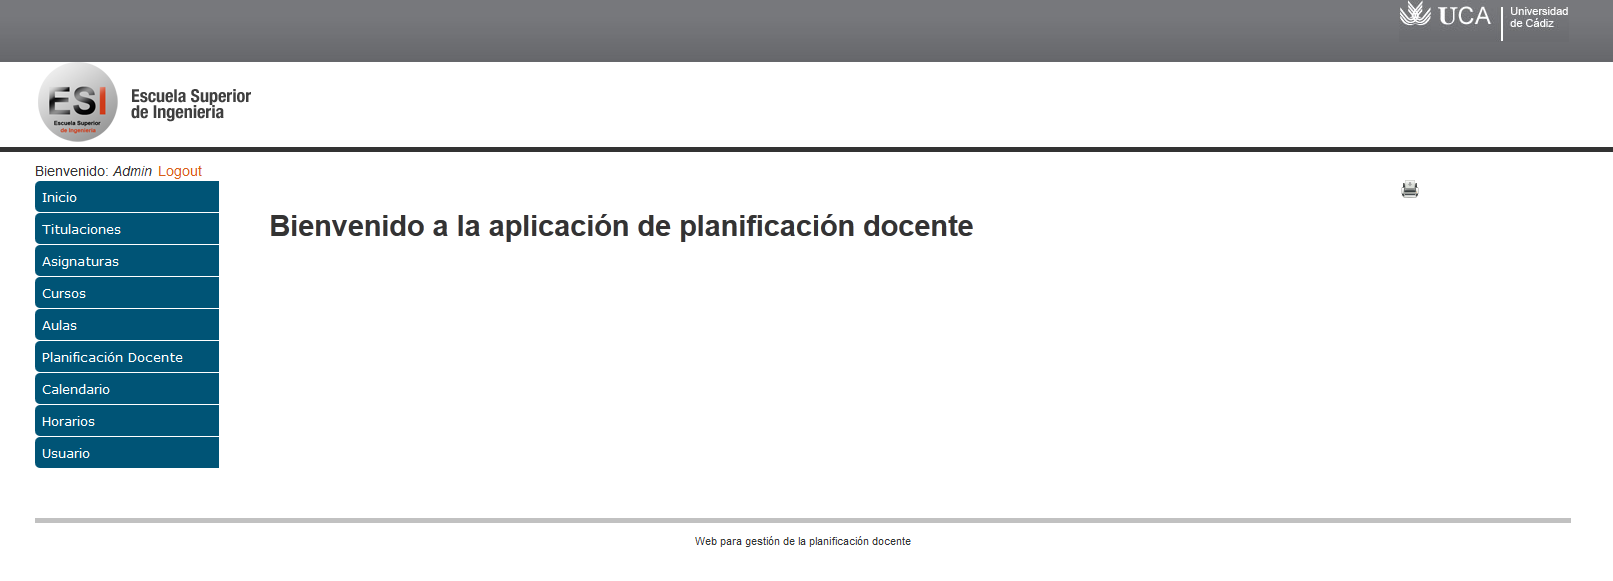
\includegraphics[scale=0.40]{./layout.png}
  \end{center}
\caption{Captura de la estructura de una página}
\end{figure}

En esta estructura tenemos un menú a la izquierda, una cabecera y un pié de página, además de un panel sobre el menú que indica el usuario que está conectado y permite su salida del sistema.\\

Todas las páginas siguen un estilo similar, por ejemplo una página que contiene una tabla de elementos, como esta con el listado de titulaciones:

\begin{figure}[H] 
  \label{captura-index-titulaciones} 
	\begin{center}
    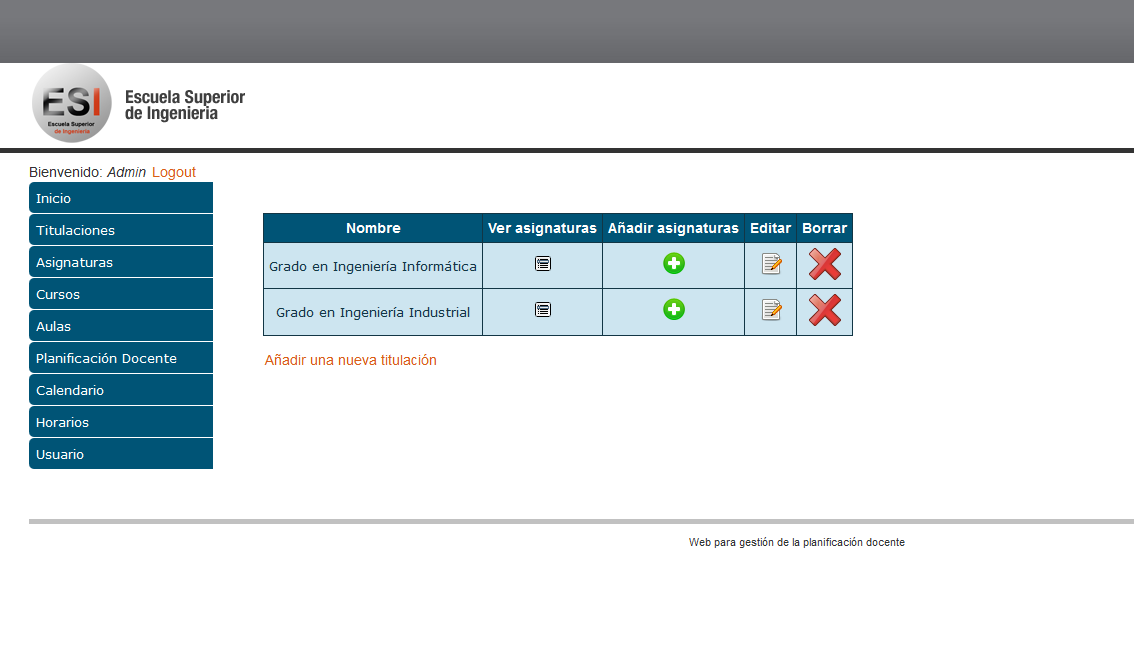
\includegraphics[scale=0.57]{./index-titulaciones.png}
  \end{center}
\caption{Captura del listado de titulaciones}
\end{figure}

La parte central del sistema es la gestión de horarios, para ello es necesaria una interacción sencilla con el usuario a la hora de construirlos y que no se convierta en una labor tediosa de realizar. Por ello se pensó que lo más sencillo sería arrastrar las asignaturas al lugar deseado en el horario, es decir, lo más intuitivo posible, esto es lo que veríamos en una de las páginas de configuración de horarios:

\begin{figure}[H] 
  \label{captura-horarios} 
	\begin{center}
    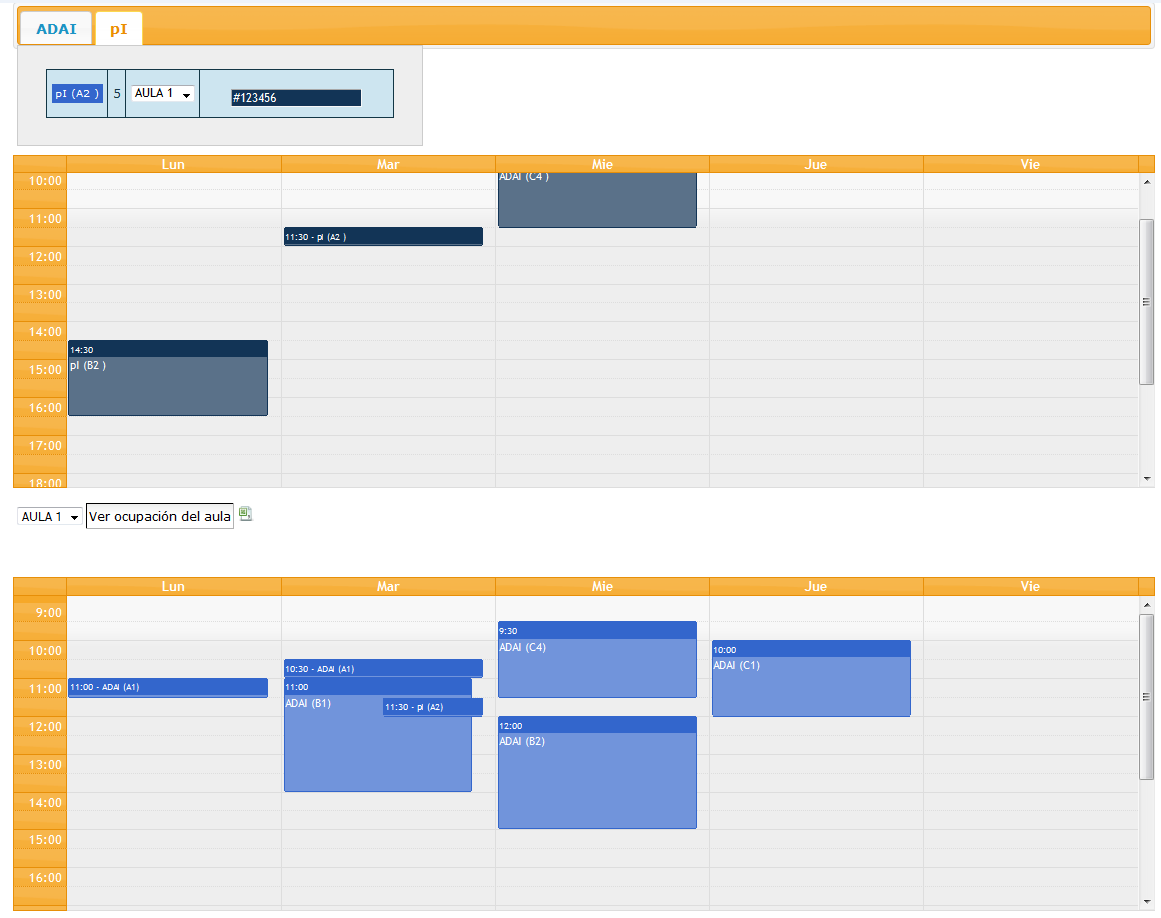
\includegraphics[scale=0.57]{./edit-horario.png}
  \end{center}
\caption{Captura de página de horarios}
\end{figure}

Tenemos tres partes diferenciadas en esta vista, un cuadro superior con las asignaturas aun no asignadas, que se podrán arrastrar al horario. Otra central con el horario de ese grupo, y otro bloque en la parte inferior en el que podemos ver la ocupación del aula que seleccionemos.
\paragraph{}
A la hora de asignar los slots en el horario hay que tener en cuenta diversos factores, como por ejemplo si el aula está ocupada, o si las asignaturas son solapables, para ello cada vez que se arrastra una asignatura al horario se hace una comprobación mediante la llamada a un servicio, devolviendo el resultado y dependiendo de si es satisfactorio o no, dejar la asignatura en su lugar o deshacer el cambio. Para deshacer el cambio, la API del plugin {\em FullCalendar} proporciona una función para invertir el proceso de la última acción realizada, eso hace el trabajo algo más sencillo.

%%%%%%%%%%%%%%%%%%%%%%%%%%%%%%%%%%%%%%%%%%%%%%%%%%%%%%%%%%%%%%%%%%%%%%%%%%%%%%
%%%%%%%%%%%%%%%%%%%%%%%%%%%%%%%%%TECNOLOGIAS%%%%%%%%%%%%%%%%%%%%%%%%%%%%%%%%%%
%%%%%%%%%%%%%%%%%%%%%%%%%%%%%%%%%%%%%%%%%%%%%%%%%%%%%%%%%%%%%%%%%%%%%%%%%%%%%%
\section{Tecnologías implicadas}
\paragraph{}
Para la realización del proyecto se han utilizado una serie de tecnologías y aplicaciones software, algunas ya mencionadas en este resumen. A continuación se enumerarán todas ellas.

\subsection{Lenguaje de programación}

se decide utilizar PHP, al ser uno de los lenguajes más extendidos en este tipo de desarrollo y ser uno de los que más se asemeja a la sintaxis de C, que es el lenguaje del que tenemos mayor base gracias a la carrera.
\paragraph{}
Además otra de las razones es su extensa documentación y su gran cantidad de librerías disponibles para extender el lenguaje.
\paragraph{}
También es importante destacar que ya que queríamos utilizar un framework que usara la arquitectura MVC.
\paragraph{}
De entre ellos se decide usar Codeigniter, al ser probablemente el más ligero de todos, lo que hace que sea el más rápido comparándolo a otros frameworks, siendo la velocidad un punto crítico en esta clase de librerías. 

\subsection{Entorno de desarrollo}
Otra elección importante es el entorno de desarrollo de código, ya que según la elección que hagamos, puede favorecer nuestra productividad o hacernos más lentos en nuestro trabajo. Aquí existe la posibilidad de decantarse por un simple editor de código o bien utilizar un entorno de desarrollo integrado (IDE), con múltiples herramientas que nos ayudan en nuestro trabajo. Nosotros nos decantamos por la segunda opción.
\paragraph{}
Se decide utilizar {\em NetBeans}, un entorno pensado inicialmente para el desarrollo Java, pero adaptado a otros lenguajes. NetBeans proporciona entre otras cosas autocompletado de código y un debugger muy completo que nos ayuda a encontrar errores en el código.

\subsection{Redacción de la memoria y resumen}

Para la realización de la memoria se ha utilizado \LaTeX, que es un lenguaje de marcado para la composición de textos científicos. Es una herramienta realmente fácil de usar y que da como resultado documentos de una gran calidad tipográfica, bastante más difícil de obtener con un procesador de textos normal.

\subsection{Ediciones rápidas de código}

A veces es necesario hacer ediciones rápidas de código para lo que no se ve necesario y productivo abrir el IDE, para ello se ha utilizado {\em Emacs}, un completo editor multiplataforma que se encuentra en el proyecto GNU y que dándole un uso adecuado puede ser tan potente como un IDE.

\subsection{Herramienta UML}

Para la creación de los diagramas UML se utilizó {\em BoUML}, que permite realizar todo tipo de diagrama dentro del estándar UML 2. Incluso provee una herramienta de generación de código para múltiples lenguajes.

\subsection{Planificación}

Para la gestión de la planificación de recursos se ha utilizado el software gratuito {\em Planner}, la elección se realizó ya que se había utilizado en otros proyectos y la experiencia fue satisfactoria.

%%%%%%%%%%%%%%%%%%%%%%%%%%%%%%%%%%%%%%%%%%%%%%%%%%%%%%%%%%%%%%%%%%%%%%%%%%%%%%
%%%%%%%%%%%%%%%%%%%%%%%%%%%%%%%%%%CONCLUSIONES%%%%%%%%%%%%%%%%%%%%%%%%%%%%%%%%
%%%%%%%%%%%%%%%%%%%%%%%%%%%%%%%%%%%%%%%%%%%%%%%%%%%%%%%%%%%%%%%%%%%%%%%%%%%%%%
\section{Conclusiones}

En este capítulo se comentarán las conclusiones personales alcanzadas, así como las posibles ampliaciones futuras que se le podrían hacer a la aplicación.

\subsection{Opinión personal}

Con este proyecto se han abarcado aspectos tanto de software de gestión como de aplicación web, conocimientos que durante la carrera se dan de forma muy básica, por lo que proyectos como este pueden ayudarme a ampliar conocimientos para desarrollos y trabajos futuros.
\paragraph{}
Realmente es la primera vez que me enfrento a un desarrollo web relativamente grande, ya que mi conocimiento y experiencia no pasaba de la realización de algunas páginas estáticas mediante HTML. Este es, por tanto, el primer acercamiento real al lenguaje PHP, del que he descubierto su potencia en este proyecto. Es cierto que podría haber evitado usar algún framework y utilizar simplemente el lenguaje sin ninguna ayuda, pero creo que sólo hubiera hecho la labor más tediosa y aburrida, y considero que el uso de un framework debería ser considerado obligatorio por cualquier programador a la hora de realizar una aplicación web, sea en PHP o en cualquier otro lenguaje.
\paragraph{}
En cuanto a JavaScript, si bien es cierto que ya lo había usado alguna otra vez, realmente nunca había probado alguna librería como  {\em jQuery}, y me ha sorprendido gratamente su potencia y facilidad de uso, y lo que se puede hacer mejorando notablemente la experiencia del usuario.
\paragraph{}
En cuanto a los sistemas de control de versiones, ya había tenido experiencia con {\em Subversion}, pero Git sorprende por su versatilidad, mostrándose mucho más fuerte a la hora de realizar desarrollos colaborativos. Se utilizó {\em GitHub} como servidor {\em Git}, ya que disponía de una amplia comunidad de usuarios y parecía ser de los más recomendados en la web, además de que disponía de un sistema de seguimiento de tareas muy bueno y fácil de usar.
\paragraph{}
En cuanto a \LaTeX no es la primera vez que lo he usado, pero esta memoria me ha servido para ampliar un poco más mi conocimiento de este lenguaje.






%%%%%%%%%%%%%%%%%%%%%%%%%%%%%%%%%%%%%%%%%%%%%%%%%%%%%%%%%%%%%%%%%%%%%%%%%%%%%%
%%%%%%%%%%%%%%%%%%%%%%%%%%%%%MEJORAS Y AMPLIACIONES%%%%%%%%%%%%%%%%%%%%%%%%%%%%
%%%%%%%%%%%%%%%%%%%%%%%%%%%%%%%%%%%%%%%%%%%%%%%%%%%%%%%%%%%%%%%%%%%%%%%%%%%%%%

\section{Ampliaciones futuras}
\paragraph{}
Este proyecto está sujeto a cambios, ya que es posible que cambie la forma en la que se plantea la planificación docente de una asignatura, y aunque la aplicación se ha intentado parametrizar lo máximo posible para poder personalizar muchos aspectos, es posible que sea necesario realizar cambios.
\paragraph{}
Entre las posibles ampliaciones que se pueden hacer está el que un alumno pueda loguearse con su usuario habitual del campus virtual, integrándolo con el LDAP de la Universidad, no se ha hecho debido a que el objetivo principal de la aplicación es ser usada por un usuario planificador para la configuración, teniendo el alumno una funcionalidad mínima.
\paragraph{}
Otra posible mejora sería una cierta automatización en la creación de los horarios, por ejemplo proponiendo un profesor su horario preferente y generándose el mejor horario posible, pudiendo ser modificado luego. En este aspecto también estaria bien la posibilidad de que un alumno propusiera una configuración mejor para un horario.

\figura{gantt1.PNG}{scale=0.6, angle=90}{Diagrama de Gannt. Desarrollo del
  proyecto 1/2}{fig:gannt1}{H}

\figura{gantt2.PNG}{scale=0.5, angle=90}{Diagrama de Gannt. Desarrollo del
  proyecto 1/2}{fig:gannt2}{H}

%%%%%%%%%%%%%%%%%%%%%%%%%%%%%%%%%%%%%%%%%%%%%%%%%%%%%%%%%%%%%%%%%%%%%%%%%%%%%%
%%%%%%%%%%%%%%%%%%%%%%%%%%%%%%%%%%BIBLIOGAFIA%%%%%%%%%%%%%%%%%%%%%%%%%%%%%%%%
%%%%%%%%%%%%%%%%%%%%%%%%%%%%%%%%%%%%%%%%%%%%%%%%%%%%%%%%%%%%%%%%%%%%%%%%%%%%%%
%\addcontentsline{toc}{chapter}{Bibliografia y referencias}
\begin{thebibliography}{99}
\bibitem{Codeigniter_userguide}Codeigniter user guide. \url{http://codeigniter.com/user_guide}.
\bibitem{jQuery_docs} Documentación jQuery. \url{http://docs.jquery.com/}.
\bibitem{fpdf_docs} Documentación librería FPDF. \url{http://www.fpdf.org/en/doc/index.php}.
\bibitem{php_docs} Documentación oficial PHP. \url{http://es.php.net/manual/es/}.
\bibitem{jquery_book} Castledine, Earle. \emph{jQuery. Novice to ninja. ISBN: 978-0-9805768-5-6}. Sitepoint, 2010.
\bibitem{Wikibooks} Wikibooks. The book of \LaTeX. \url{http://en.wikibooks.org/wiki/LaTeX/}.
\bibitem{Web_Latex}Guía para la generación de la memoria del Proyecto Fin de Carrera.\\ \url{http://osl2.uca.es/wikiformacion/index.php/LaTeX_para_Proyecto_Fin_de_Carrera}.
\bibitem{design_patterns} Gamma, Erich. \emph{Design Patterns. Elements of Reusable Object-Oriented Software. ISBN: 0-201-63361-2}. Addison-Wesley, 1995
\bibitem{TDD_book} Beck, Kent. \emph{Test-Driven Development By Example. ISBN: 0-321-14653-0}. Addison-Wesley, 2003
\end{thebibliography}

\end{document}